\section{Results}
\label{results}

Table~\ref{yields} shows the expected number of background events and the observed data in each SR and \pt bin, for each channel. We split SR I into two bins. In the $\Pe\Pgm$ and $\Pgm\Pgm$ channels, these bins are in the leading muon \pt, and in the $\Pe\Pe$ channel, these bins are in the leading electron \pt. The \pt bins are chosen such that the high-\pt bin contains ${<}1$ background event, which increases the sensitivity to small lifetimes and large masses. The observed number of events are consistent with the predicted amount of background.
% \FIXME : why not define the pt bins earlier?

\begin{table}
\renewcommand{\arraystretch}{1.3}
\noindent \centering{}
\topcaption{The number of estimated background and observed events in each channel and SR. For each estimate, the total uncertainty is given. The \pt boundaries that separate the low- and high-\pt bins of SR I are listed in Table~\ref{pt_bins}.}
\label{yields}
\begin{tabular}{llllll}
\hline
 & SR I, & SR I,  &  &  & \\
 & low \pt & high \pt & SR II & SR III & SR IV \\
 & bin & bin &  & & \\
\hline
\textit{2016 $\Pe\Pgm$}\\
- estimated        & $3.8^{+4.8}_{-3.8}$    & $0.41^{+0.53}_{-0.41}$ & $0.09^{+0.12}_{-0.09}$ & $0.15\pm0.15$ & $0.003^{+0.004}_{-0.003}$\\
- observed         & 8 & 1 & 0 & 0 & 0\\

\textit{2017+2018 $\Pe\Pgm$}\\
- estimated        & $38\pm13$          & $0.75^{+0.41}_{-0.34}$ & $0.23^{+0.27}_{-0.23}$ & $0.71^{+0.76}_{-0.71}$ & $0.01^{+0.02}_{-0.01}$\\
- observed         & 28 & 3 & 0 & 1 & 0\\

\textit{2016 $\Pe\Pe$}\\
- estimated        & $18\pm11$  & $0.22^{+0.17}_{-0.16}$ & $0.51^{+1.02}_{-0.51}$ & $0.43^{+0.85}_{-0.43}$ & $0.01^{+0.02}_{-0.01}$\\
- observed         & 40 & 0 & 0 & 1 & 0\\

\textit{2017+2018 $\Pe\Pe$}\\
- estimated        & $62^{+18}_{-17}$       & $0.85^{+0.33}_{-0.35}$ & $2.8\pm1.1$            & $3.6\pm1.4$            & $0.24^{+0.10}_{-0.09}$\\
- observed         & 48 & 0 & 1 & 4 & 0\\

\textit{2016 $\Pgm\Pgm$}\\
- estimated        & $7.4\pm3.0$            & $0.25\pm0.11$          & $0.17\pm0.11$          & $0.19\pm0.12$          & $0.01\pm0.01$\\
- observed         & 15 & 0 & 0 & 1 & 0\\

\textit{2017+2018 $\Pgm\Pgm$}\\
- estimated        & $3.5\pm1.5$            & $0.69\pm0.31$          & $0.08^{+0.12}_{-0.08}$ & $0.14^{+0.19}_{-0.14}$ & $0.01^{+0.02}_{-0.01}$\\
- observed         & 1 & 1 & 1 & 1 & 0\\
\hline
\end{tabular}
\end{table}


Figure~\ref{d0_d0_data} shows two-dimensional \ad distributions of data events that pass the preselection, and Fig.~\ref{d0_d0_sr_data} shows the same but for data events in the inclusive SR. Figure~\ref{d0_d0_sr_data_and_signal} shows the the same along with a representative signal point.

\begin{figure}
\centering
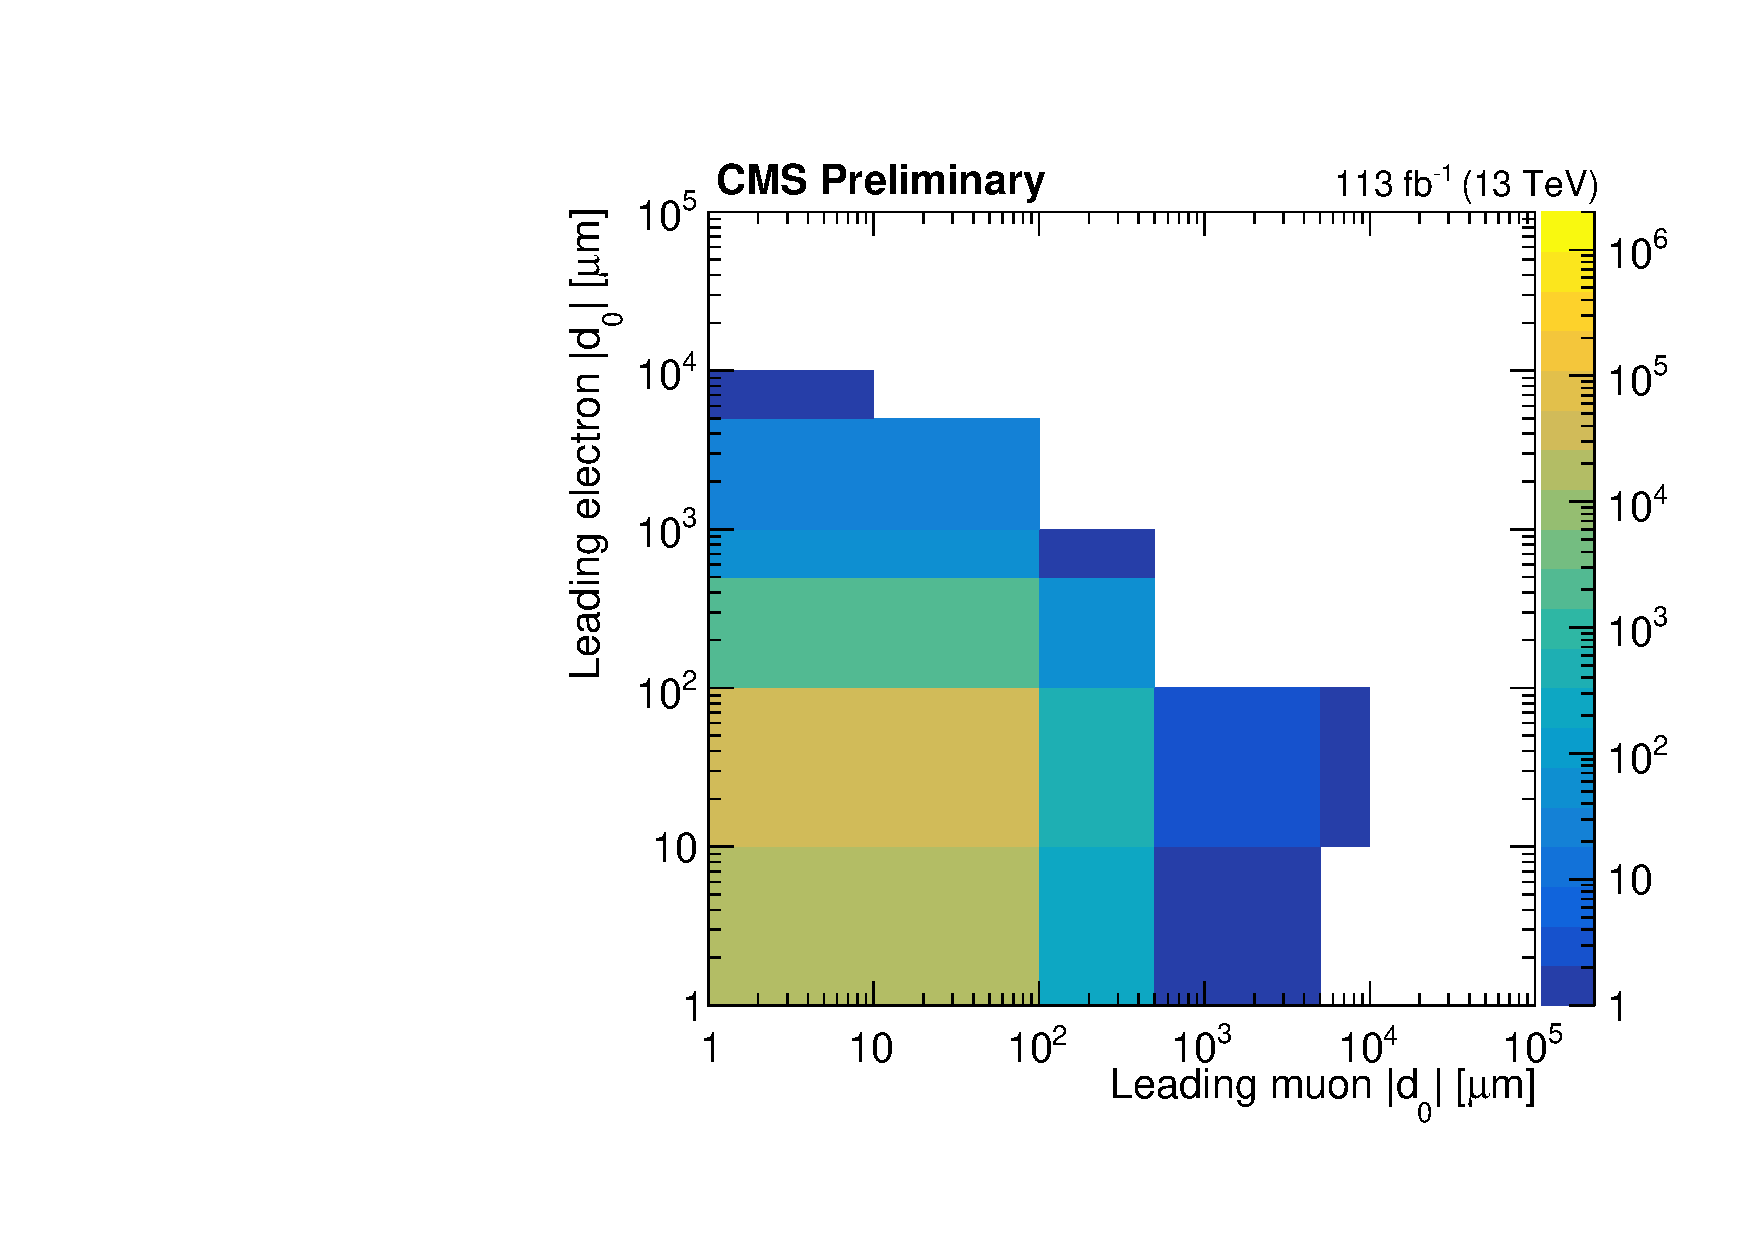
\includegraphics[width=0.32\textwidth]{figures/results/d0vsd0_emu_CMSPreliminary.pdf}
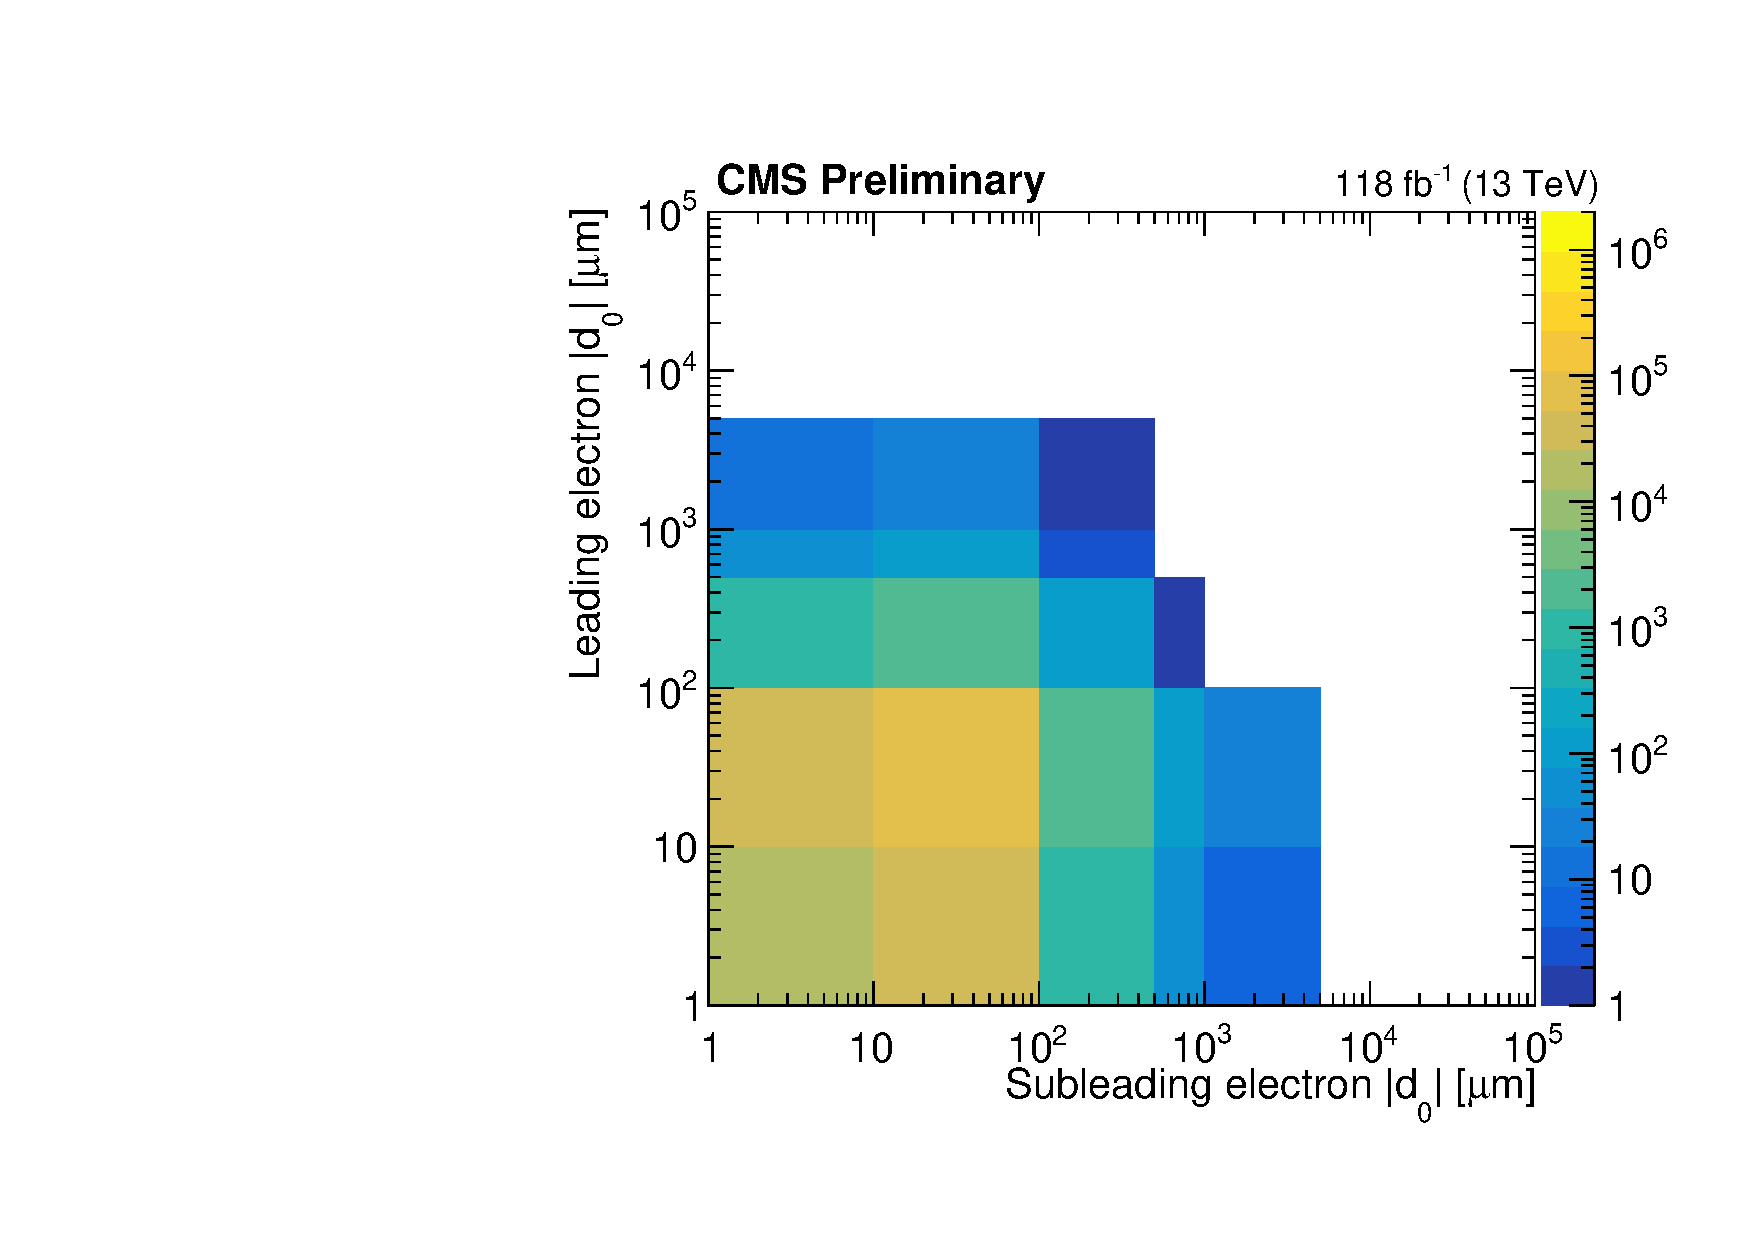
\includegraphics[width=0.32\textwidth]{figures/results/d0vsd0_ee_CMSPreliminary.pdf}
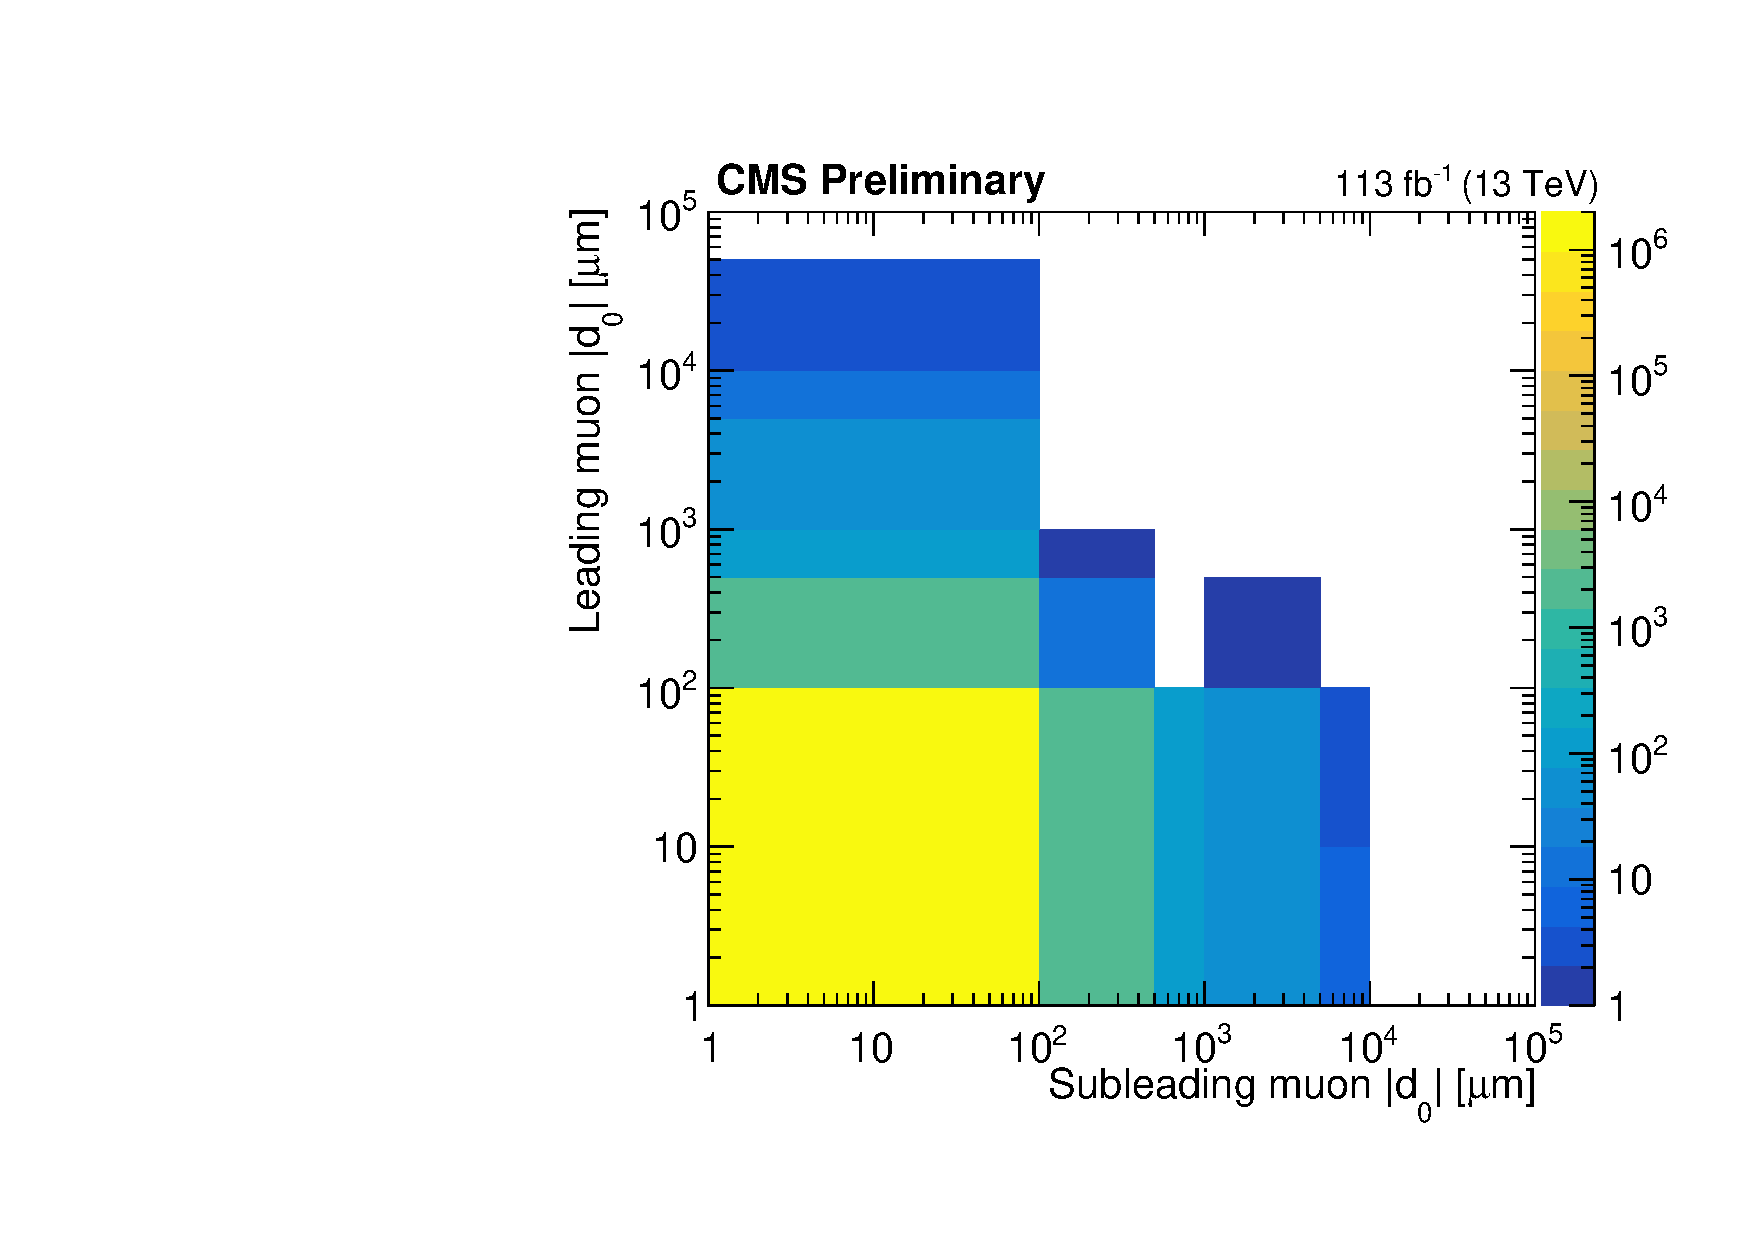
\includegraphics[width=0.32\textwidth]{figures/results/d0vsd0_mumu_CMSPreliminary.pdf}
\caption{
Two-dimensional distributions of \ada and \adb, for the events in data that pass the $\Pe\Pgm$ (left), $\Pe\Pe$ (middle), and $\Pgm\Pgm$ (right) preselection. The bins along the x and y axes contain underflow. The inclusive signal region covers the region between \SI{100}{\um} and \SI{10}{\cm} in each \ad variable shown.
}
\label{d0_d0_data}
\end{figure}

\begin{figure}
\centering
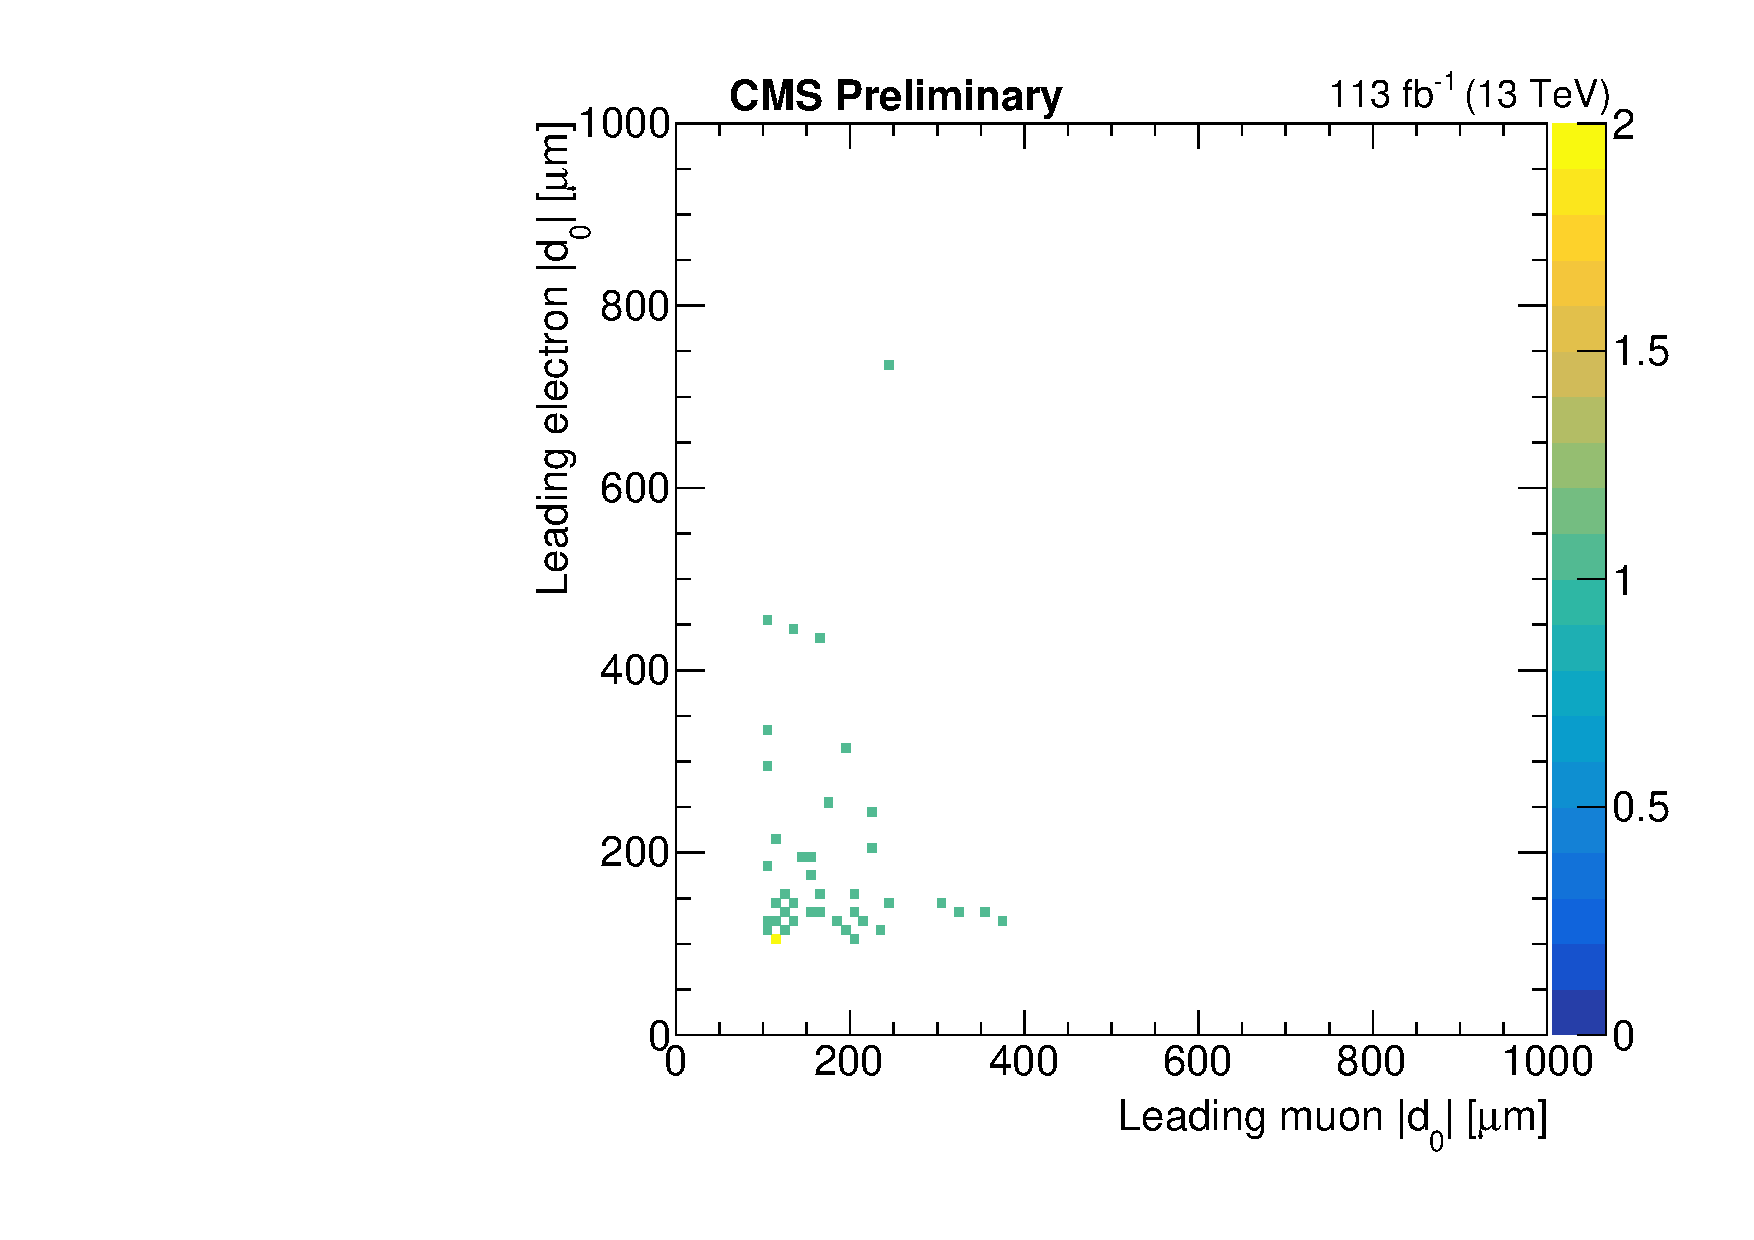
\includegraphics[width=0.31\textwidth]{figures/results/electronAbsD0[0]_vs_muonAbsD0[0]_1000um.pdf}
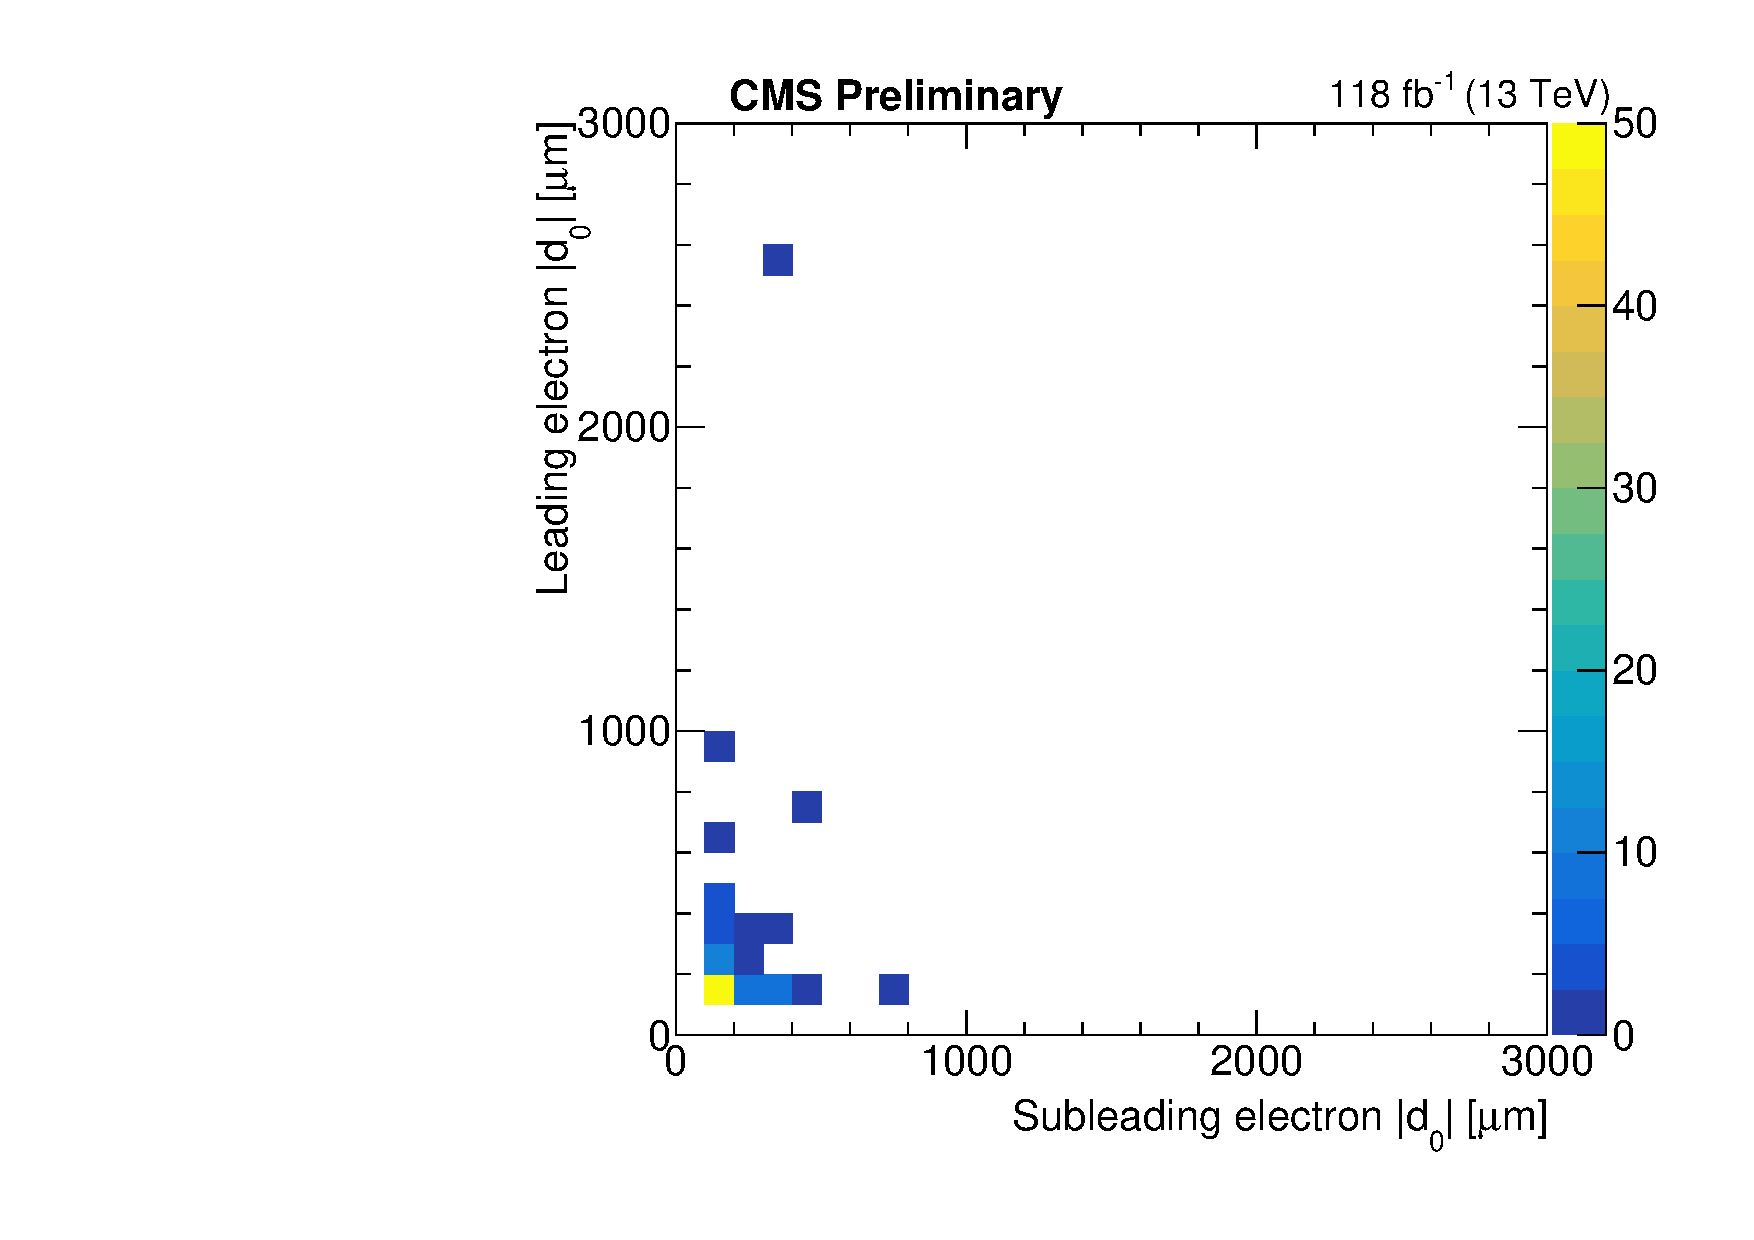
\includegraphics[width=0.31\textwidth]{figures/results/electronAbsD0[0]_vs_electronAbsD0[1]_10000um.pdf}
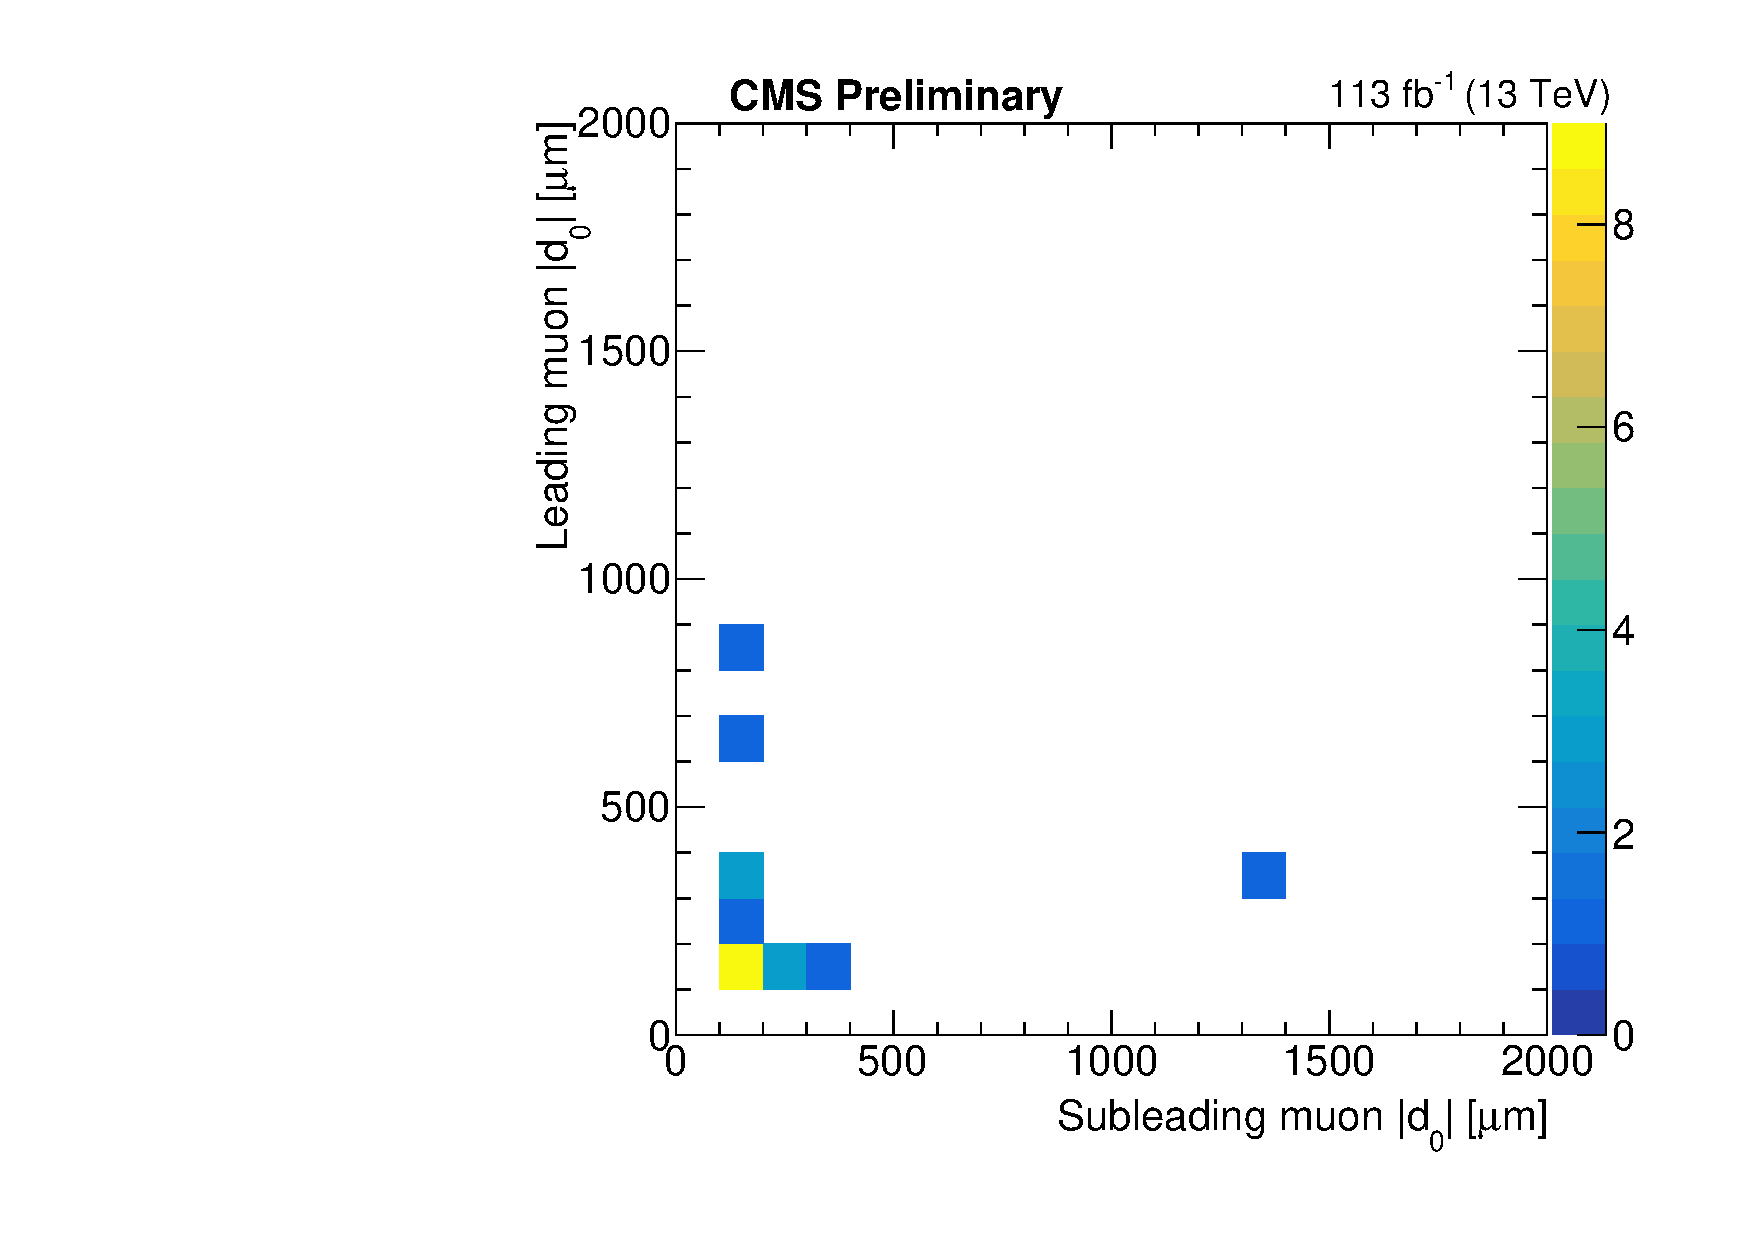
\includegraphics[width=0.31\textwidth]{figures/results/muonAbsD0[0]_vs_muonAbsD0[1]_10000um.pdf}
\caption{
Two-dimensional distributions of \ada and \adb, for data events in the inclusive SR in the $\Pe\Pgm$ (left), $\Pe\Pe$ (middle), and $\Pgm\Pgm$ (right) channels.
}
\label{d0_d0_sr_data}
\end{figure}

\subsection{Observed events}
This section provides a summary of observations recorded while examining event displays of the signal region events.

In general, the SR events appear to be SM events from the $\Pp\Pp$ collision. Specifically, we see no evidence of leptons from cosmic rays, material interactions, or signal.

In the $\Pe\Pgm$ channel, the SR events tend to have several jets and often have significant MET. Many events have muon $\phi$ values such that the muon system hits are all near the edges of detector sections or muon $\eta$ values such that the muon is near the barrel/endcap transition in the muon system. There are also a few events in which the electron and/or muon are associated with different primary vertex than their associated track.

In the $\Pe\Pe$ channel, the majority of SR events contain at least one electron with $\abs{eta} > 1.1$, where increases the probability that their $d_0$ is poorly measured. Across all three years, most events fall into one of three categories: 
\begin{enumerate}
    \item Events with two electrons that appear to be from a boosted \PZ boson, with an invariant mass between 80 and 100\GeV, opposite one or two jets
    \item Events with two electrons approximately back-to-back in $\phi$ with an invariant mass greater than 100\GeV and MET usually between 10 and 40\GeV
    \item Events that are similar to type 2 but with at least one jet and frequently MET between 70 and 110\GeV
\end{enumerate}

In the $\Pgm\Pgm$ channel, many events have an invariant mass consistent with the mass of the \PZ boson and MET less than about 60\GeV. Most of the events found in 2017 and 2018 have an invariant mass higher than than the \PZ boson mass and could be \ttbar events. Eight of the sixteen SR events in 2016 have two muons with $\phi$ values of about $\pm\pi/2$. All of the muon pairs in these eight events have an invariant mass consistent with a \PZ boson. Furthermore, the $\cos(\alpha)$ and timing distributions of these muons imply that they are not from cosmic rays. Thirteen of the sixteen muons in these eight events have only one valid pixel hit, and event displays of these events show that the muon track often passes between or at the edge of pixel modules near the place where the two halves of the pixel detector barrel are joined. We believe that this feature causes the muon $d_0$ values to be poorly measured.
% \FIXME: add some event displays

\subsection{Limits}

The data show no significant excess over background, so we set upper limits on the product of the signal production cross section ($\sigma$) and branching fraction ($\mathcal{B}$) using the ``Combine'' tool developed by the CMS Higgs working group with HybridNew limits ~\cite{Junk_CLS,Read_CLS,Cowan:2010js,CMS-NOTE-2011-005}. The ABCD estimate is performed in Combine, which has the advantage that any signal contamination in the control regions is automatically accounted for. We perform a simultaneous counting experiment in each signal region bin. Figure~\ref{limits_individual} shows the 95\% confidence level ($\CL$) upper limits on the top squark mass as a function of its lifetime.
%top squark, Higgs boson, and slepton lifetimes as a function of their masses, for each of the three channels.

The variation in the size and shape of the exclusion regions between the three channels is mostly explained by variation in signal yields between the three channels. Looking at the high-\pt bin of SR I, which is the most sensitive bin for top squarks with large masses and small lifetimes, we find that the simulated signal yield is highest in the $\Pe\Pgm$. This difference between the $\Pe\Pgm$ and same-flavor channels is a result of simple combinatorics: the two independent top squark decays will result in an $\Pe\Pgm$ final state twice as often as an $\Pe\Pe$ or $\Pgm\Pgm$ final state. In this bin, the $\Pe\Pe$ and $\Pgm\Pgm$ channel signal yields are similar. In SR IV, which drives the sensitivity for top squarks with large lifetimes, the $\Pgm\Pgm$ channel has the largest simulated signal yield when considering top squarks with lifetimes $\gtrsim10\cm$. This difference is due to the better muon reconstruction than electron reconstruction of CMS. For this same reason, the $\Pe\Pe$ channel has the smallest signal yield out of the three channels in SR IV when considering top squark lifetimes $\gtrsim10\cm$. Taking all of these effects together, we find that the $\Pe\Pgm$ channel is the most sensitive for lifetimes ${\lesssim}10\cm$ while the $\Pgm\Pgm$ channel is the most sensitive for lifetimes ${\gtrsim}10\cm$

Figure~\ref{limits_combined} shows the 95\% $\CL$ upper limits for the combination of the three channels. The top squark limits assume $\mathcal{B}(\PSQt \to \cPqb \Pl)=\mathcal{B}(\PSQt \to \cPqd \Pl)=100\%$, and each $\Pl$ has an equal probability of being an electron, a muon, or a tau lepton. The Higgs boson limits assume $\mathcal{B}(\PH \to \mathrm{S}\mathrm{S}=100\%$, and each $\Pl$ has an equal probability of being an electron or a muon. See Appendix~\ref{sec:likelihoodTests} for more information on how the likelihood handles the observed yields.
%The slepton limits assume the superpartners of the left- and right-handed leptons are mass degenerate.

\begin{figure}
\centering
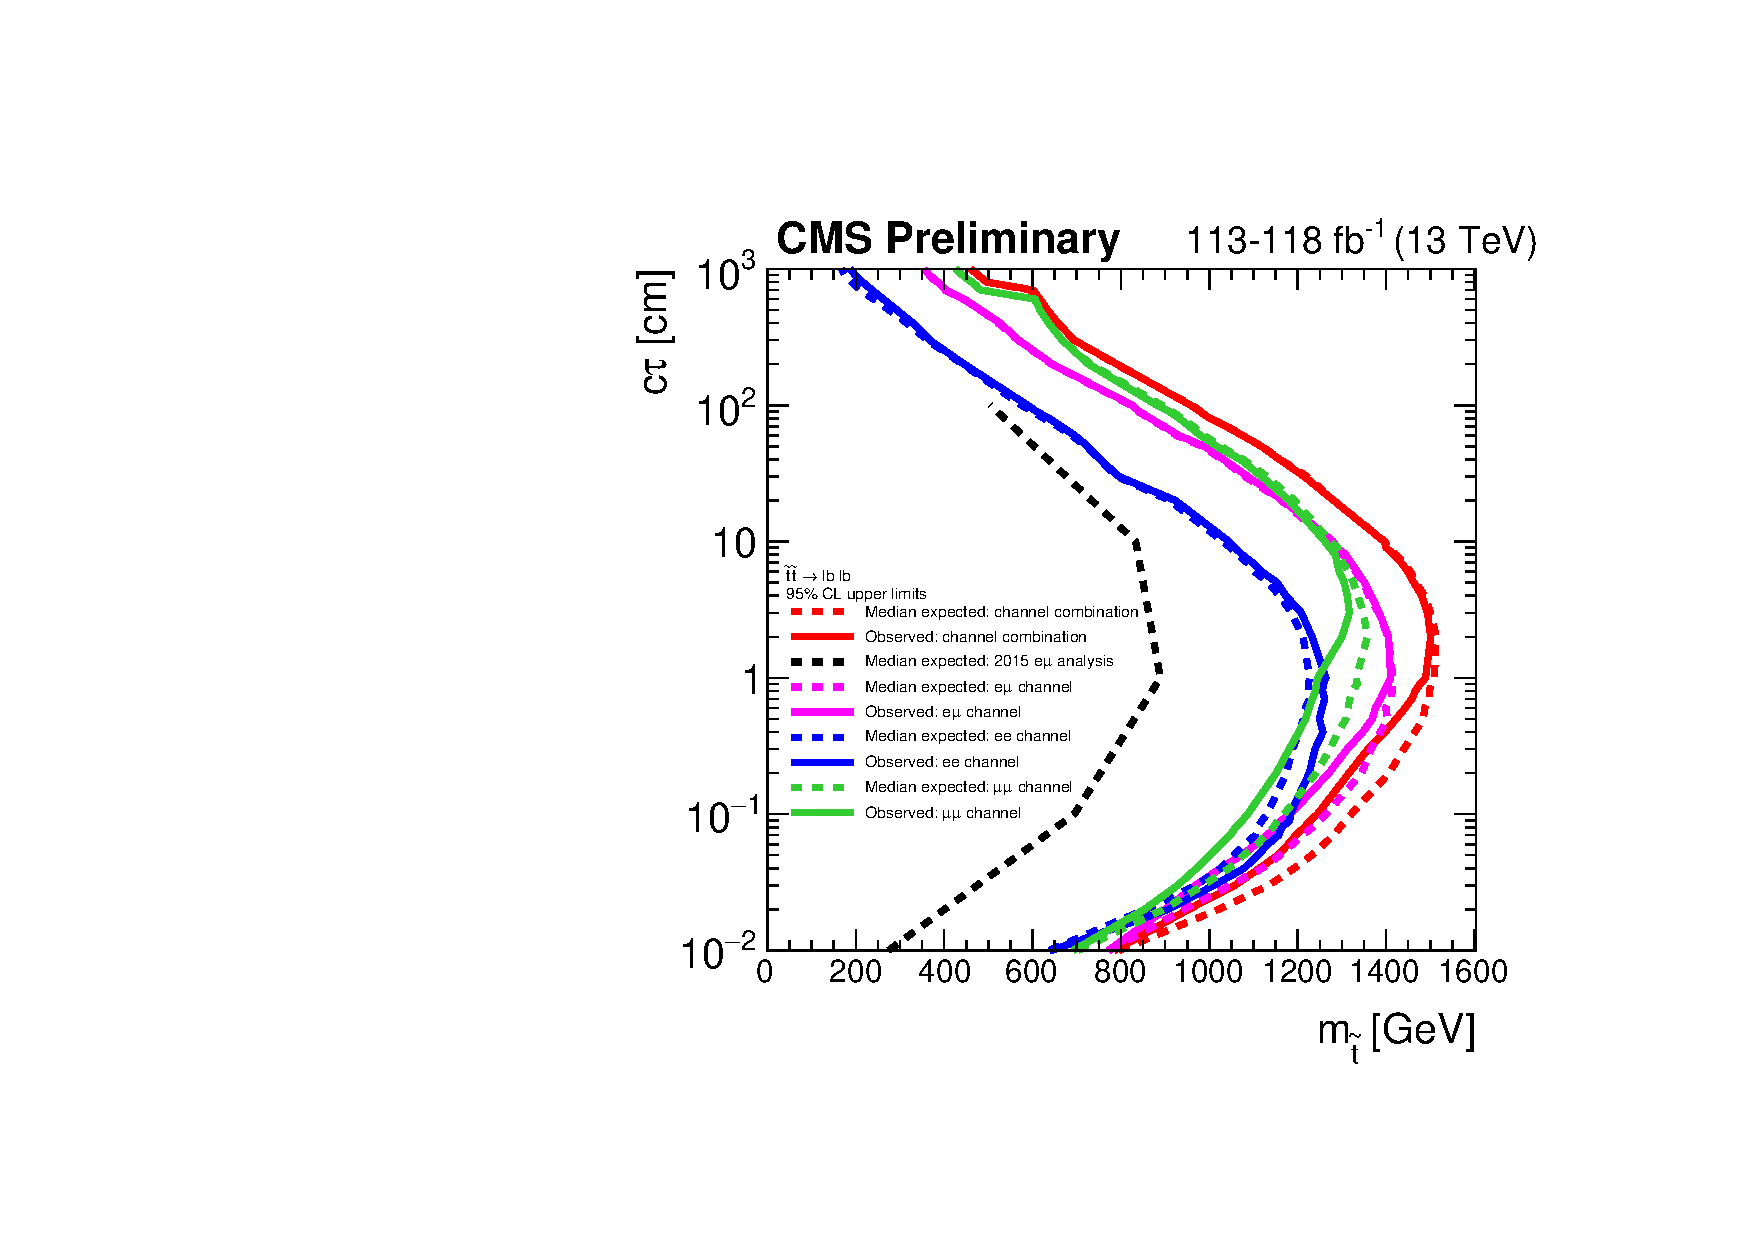
\includegraphics[width=0.65\textwidth]{figures/results/2DlimitsStopToLB.pdf}
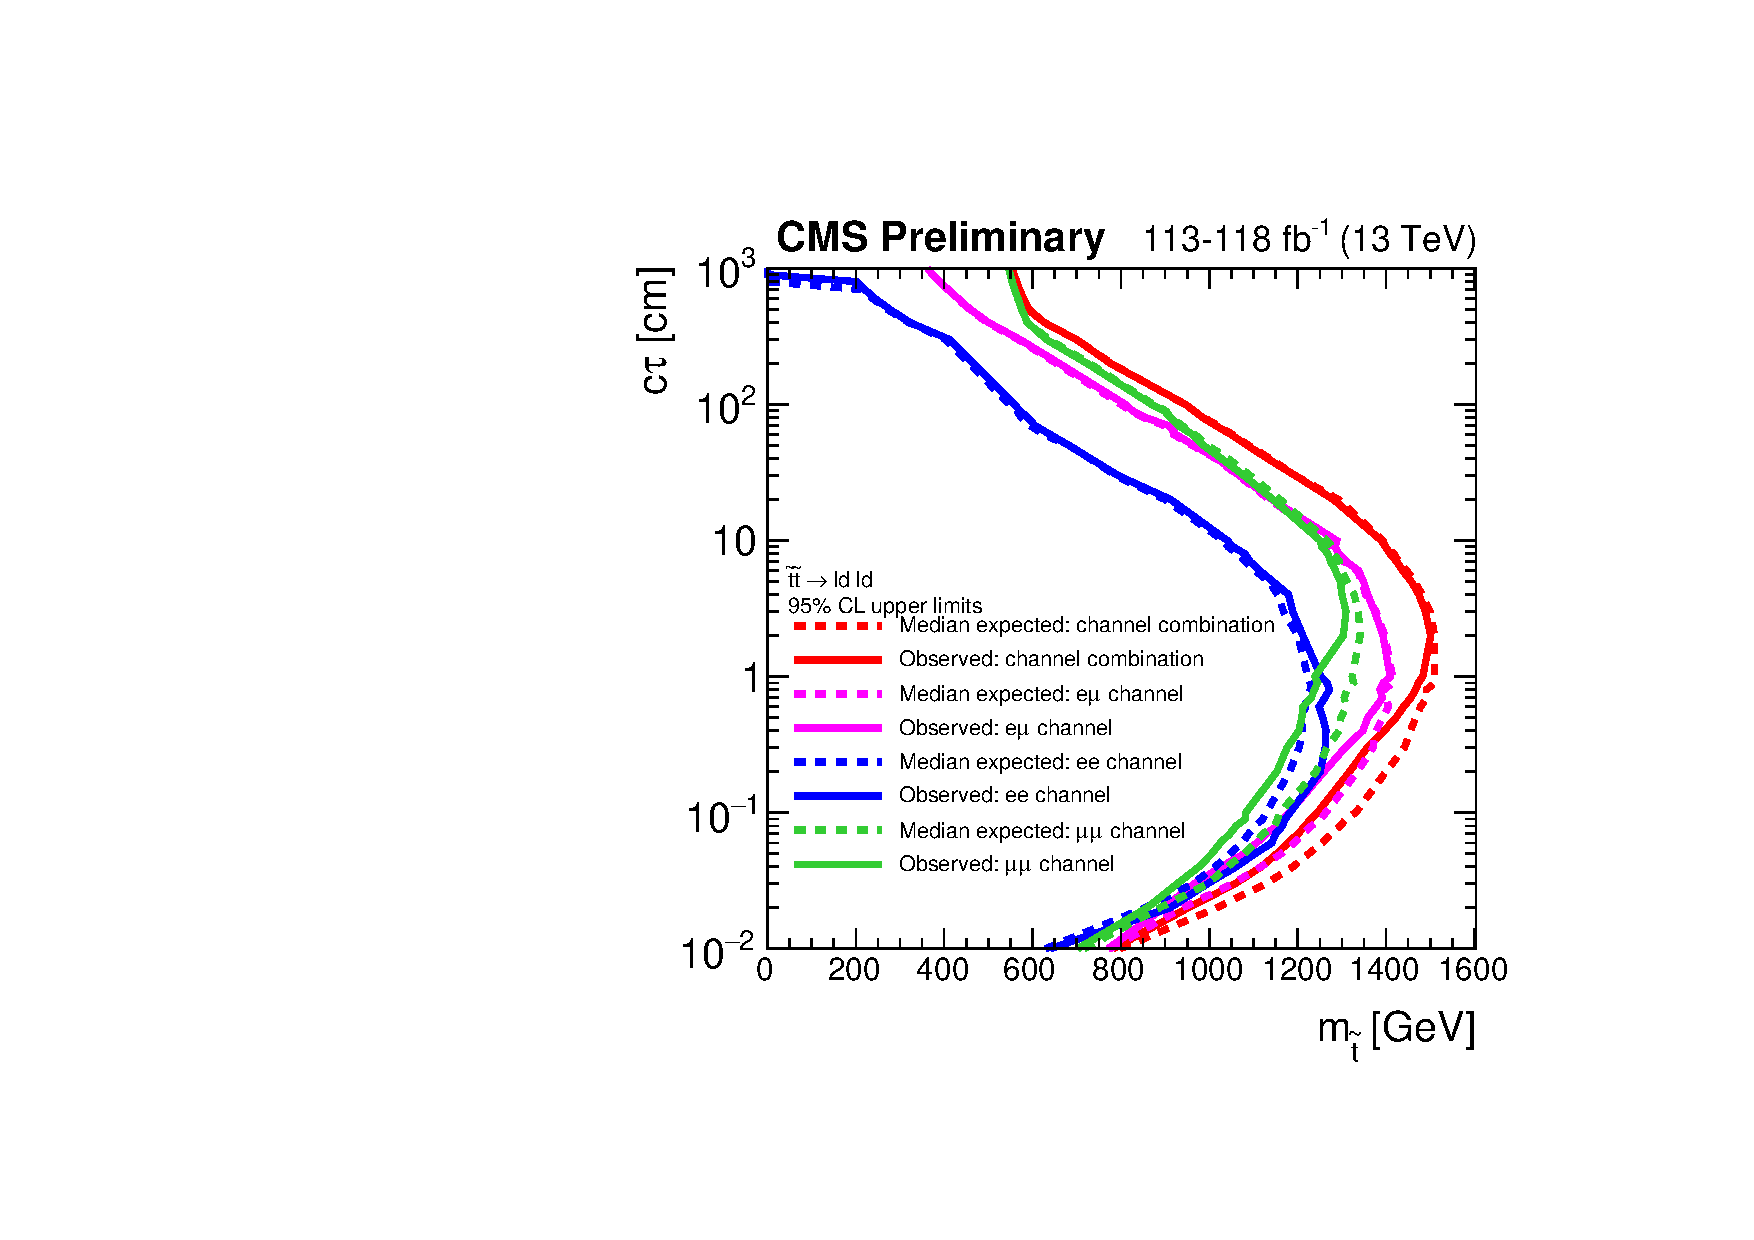
\includegraphics[width=0.65\textwidth]{figures/results/2DlimitsStopToLD.pdf}
\caption{The 95\% $\CL$ upper limits on the top squark mass ($m_{\PSQt}$) as a function of its lifetime ($c\tau$), for the $\Pe\Pgm$, $\Pe\Pe$, and $\Pgm\Pgm$ channels. The \stoptolb (top) and \stoptold (bottom) processes are shown.} 
%The $\PSQt\PASQt \to \PAl\PQb\:\Pl\PAQb $ (upper left), $\PSQt\PASQt \to \PAl\PQd\:\Pl\PAQd$ (upper right), $\PSl\PASl \to \PAl\PXXSG\:\Pl\PXXSG$ (lower left), and $\PH \to \PS\PS \to \Pl\PAl\:\Pl\PAl$ (lower right) processes are shown.}
\label{limits_individual}
\end{figure}

\begin{figure}
\centering
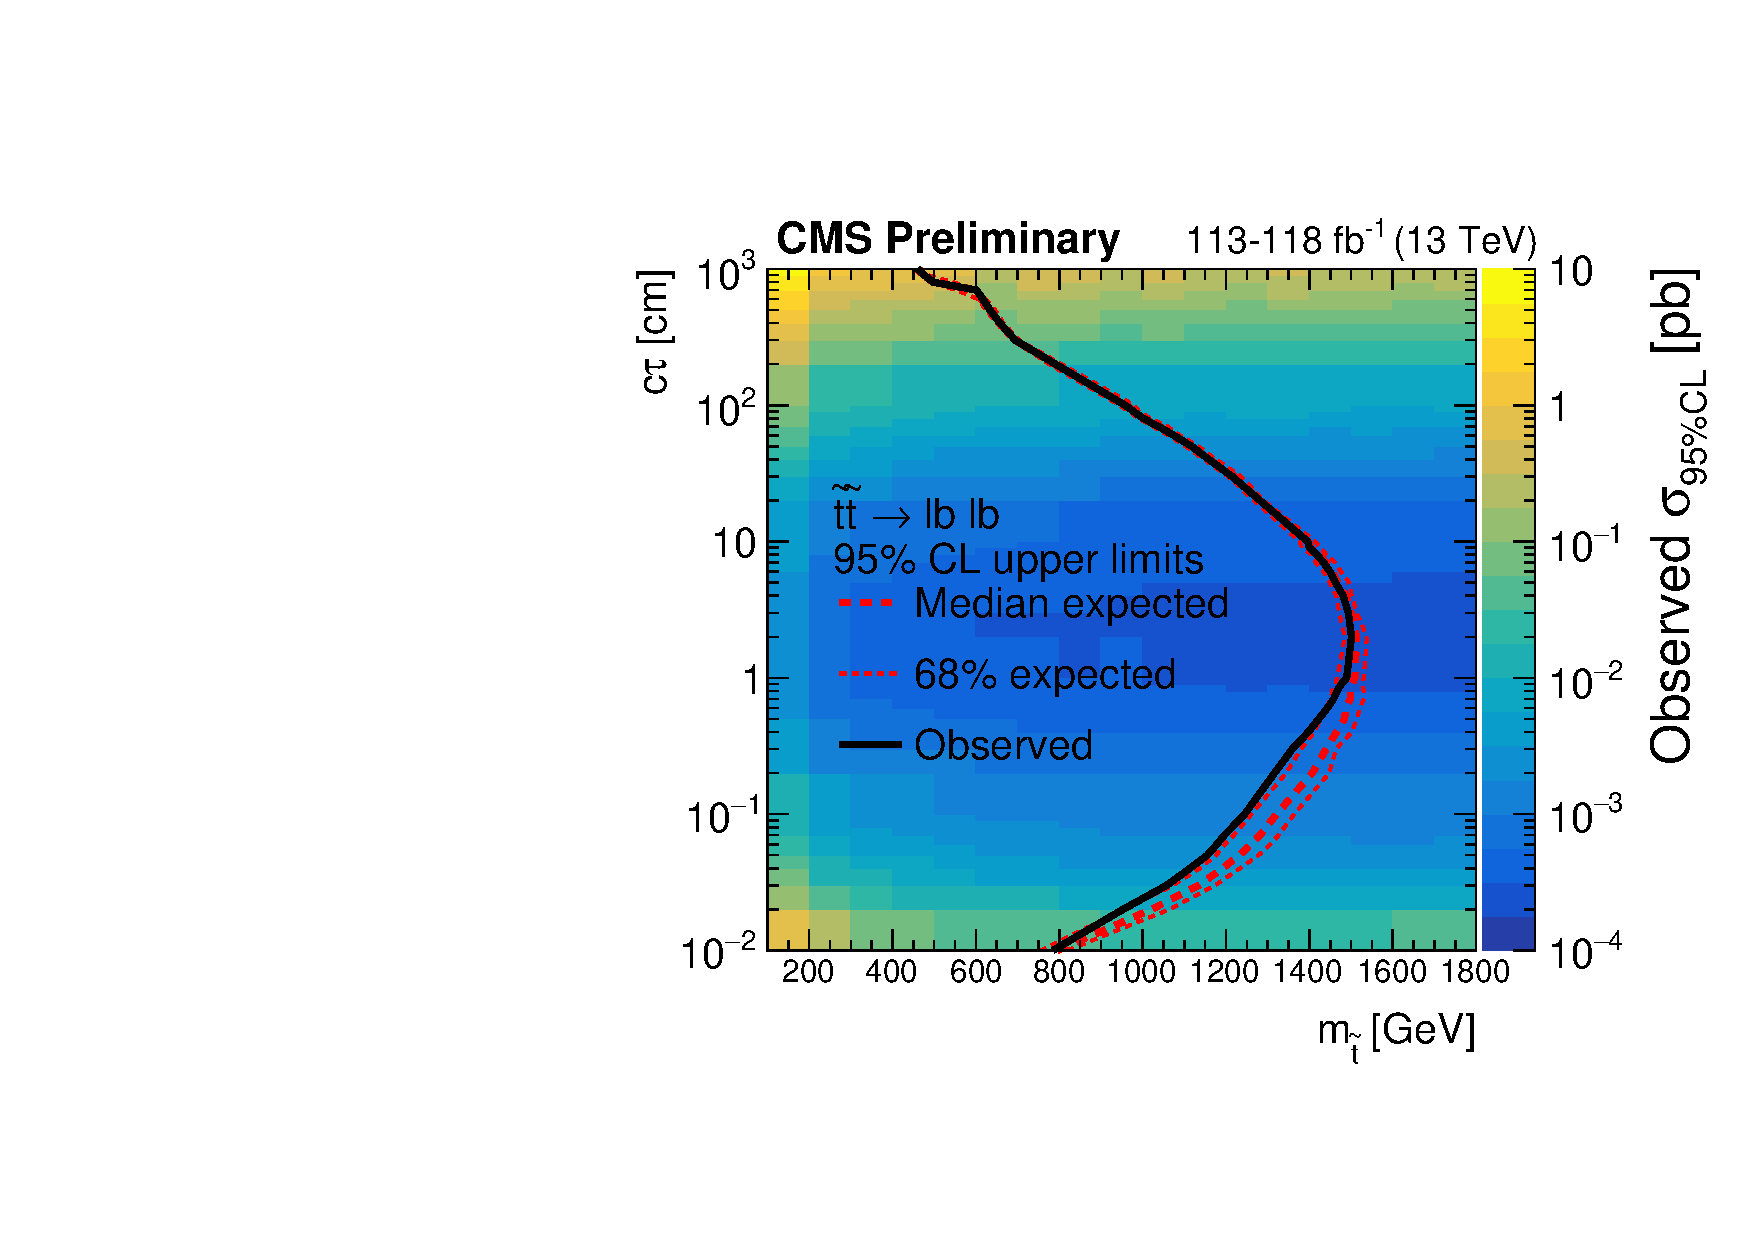
\includegraphics[width=0.65\textwidth]{figures/results/2DlimitsCombinedStopToLB.pdf}
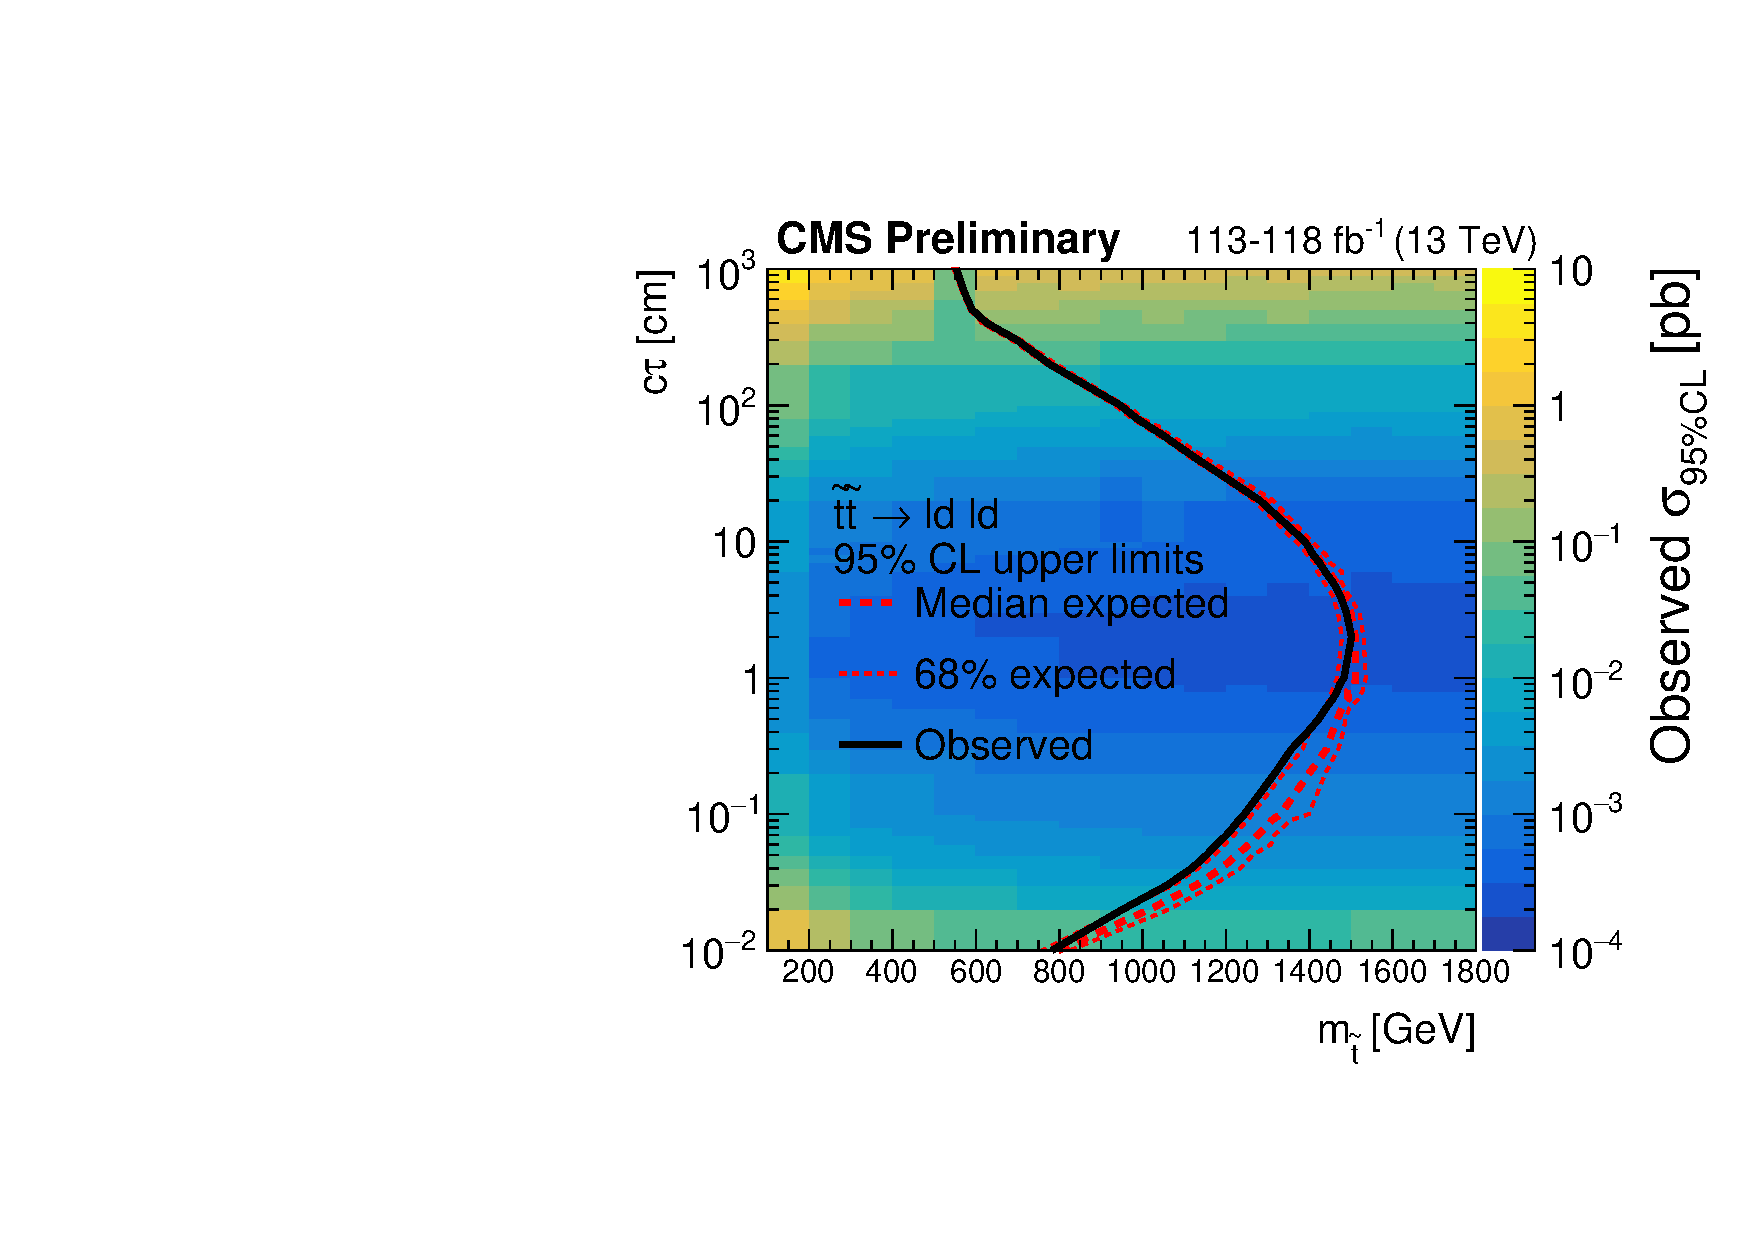
\includegraphics[width=0.65\textwidth]{figures/results/2DlimitsCombinedStopToLD.pdf}
\caption{The 95\% $\CL$ upper limits on the top squark mass ($m_{\PSQt}$) as a function of its lifetime ($c\tau$). The colors indicate the observed 95\% $\CL$ upper limit on the cross section. The \stoptolb (left) and \stoptold (right) processes are shown.} 
%The $\PSQt\PASQt \to \PAl\PQb\:\Pl\PAQb $ (upper left), $\PSQt\PASQt \to \PAl\PQd\:\Pl\PAQd$ (upper right), $\PSl\PASl \to \PAl\PXXSG\:\Pl\PXXSG$ (lower left), and $\PH \to \PS\PS \to \Pl\PAl\:\Pl\PAl$ (lower right) processes are shown.}
\label{limits_combined}
\end{figure}

\subsection{Additional likelihood tests}


\pagebreak